\subsection{SignalR}

В последнее время в веб-среде все чаще создаются веб-приложения, использующие технологии коммуникаций в реальном времени: это и простые чаты, и более сложные многопользовательские видеоконференции. Такие приложения могут использовать различные приемы работы: технологию Web Socket, опросы long polling и т.д. Для упрощения работы с коммуникациями реального времени была создана специальная библиотека под названием SignalR.

\begin{figure}[h!]
	\centering
	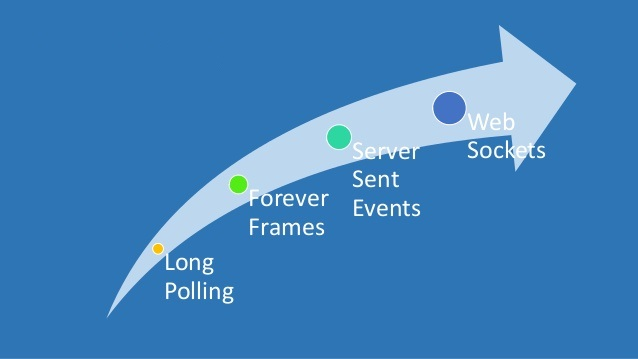
\includegraphics[scale=0.78]{signalR.jpg}
	\caption{Приоритет технологий, которые использует SignalR}
\end{figure}

SignalR использует новый протокол обмена сообщениями WebSocket, там где это возможно, и переходит на более старые протоколы, там где это необходимо. Конечно можно написать приложение напрямую используя WebSocket, но с SignalR большую часть функциональности уже не придется реализовывать. Самое главное с SignalR не надо будет беспокоиться о написании кода для поддержки старых протоколов обмена сообщениями. SignalR также избавит от необходимости обновления протокола WebSocket. И будет поддерживать приложение в целостном состоянии при переходе на новые версии.

SignalR предоставляет простой API для создания функционала, который позволяет вызывать функции JavaScript на стороне клиента из серверного кода, написанного с помощью языков платформы .NET. SignalR значительно упрощает работу с коммуникациями реального времени. Библиотека обрабатывает все подключения и автоматически рассылает сообщения всем подключенным клиентам, либо каким-нибудь специфическим клиентам.